\chapter{Measuring Beam Waist}
\label{BeamWaistAppendix}

This appendix describes techniques for characterizing the beam profile. These techniques were useful when doing the work described in Section\,\ref{optimbeamWaist} to make sure that the maximum intensity of the beam was not above a certain threshold. In this appendix, I will discuss two methods for trying to characterize the profile of the laser beam. One method was a well-known technique involving a knife. This technique worked. The other method involved a camera and did not work due to the limitations of the camera.  

\section{Knife measurements}
In order to take measurements with a knife, we block some fraction of the beam by mounting the knife on a translation stage. We then use the translation stage to move the knife perpendicular to the direction of beam propagation. At several different positions, we look at the amount of power from the beam hitting a photodiode that is placed downstream from the knife. This is illustrated in Figure\,\ref{knifeDiagram}.
\begin{figure}
\centering
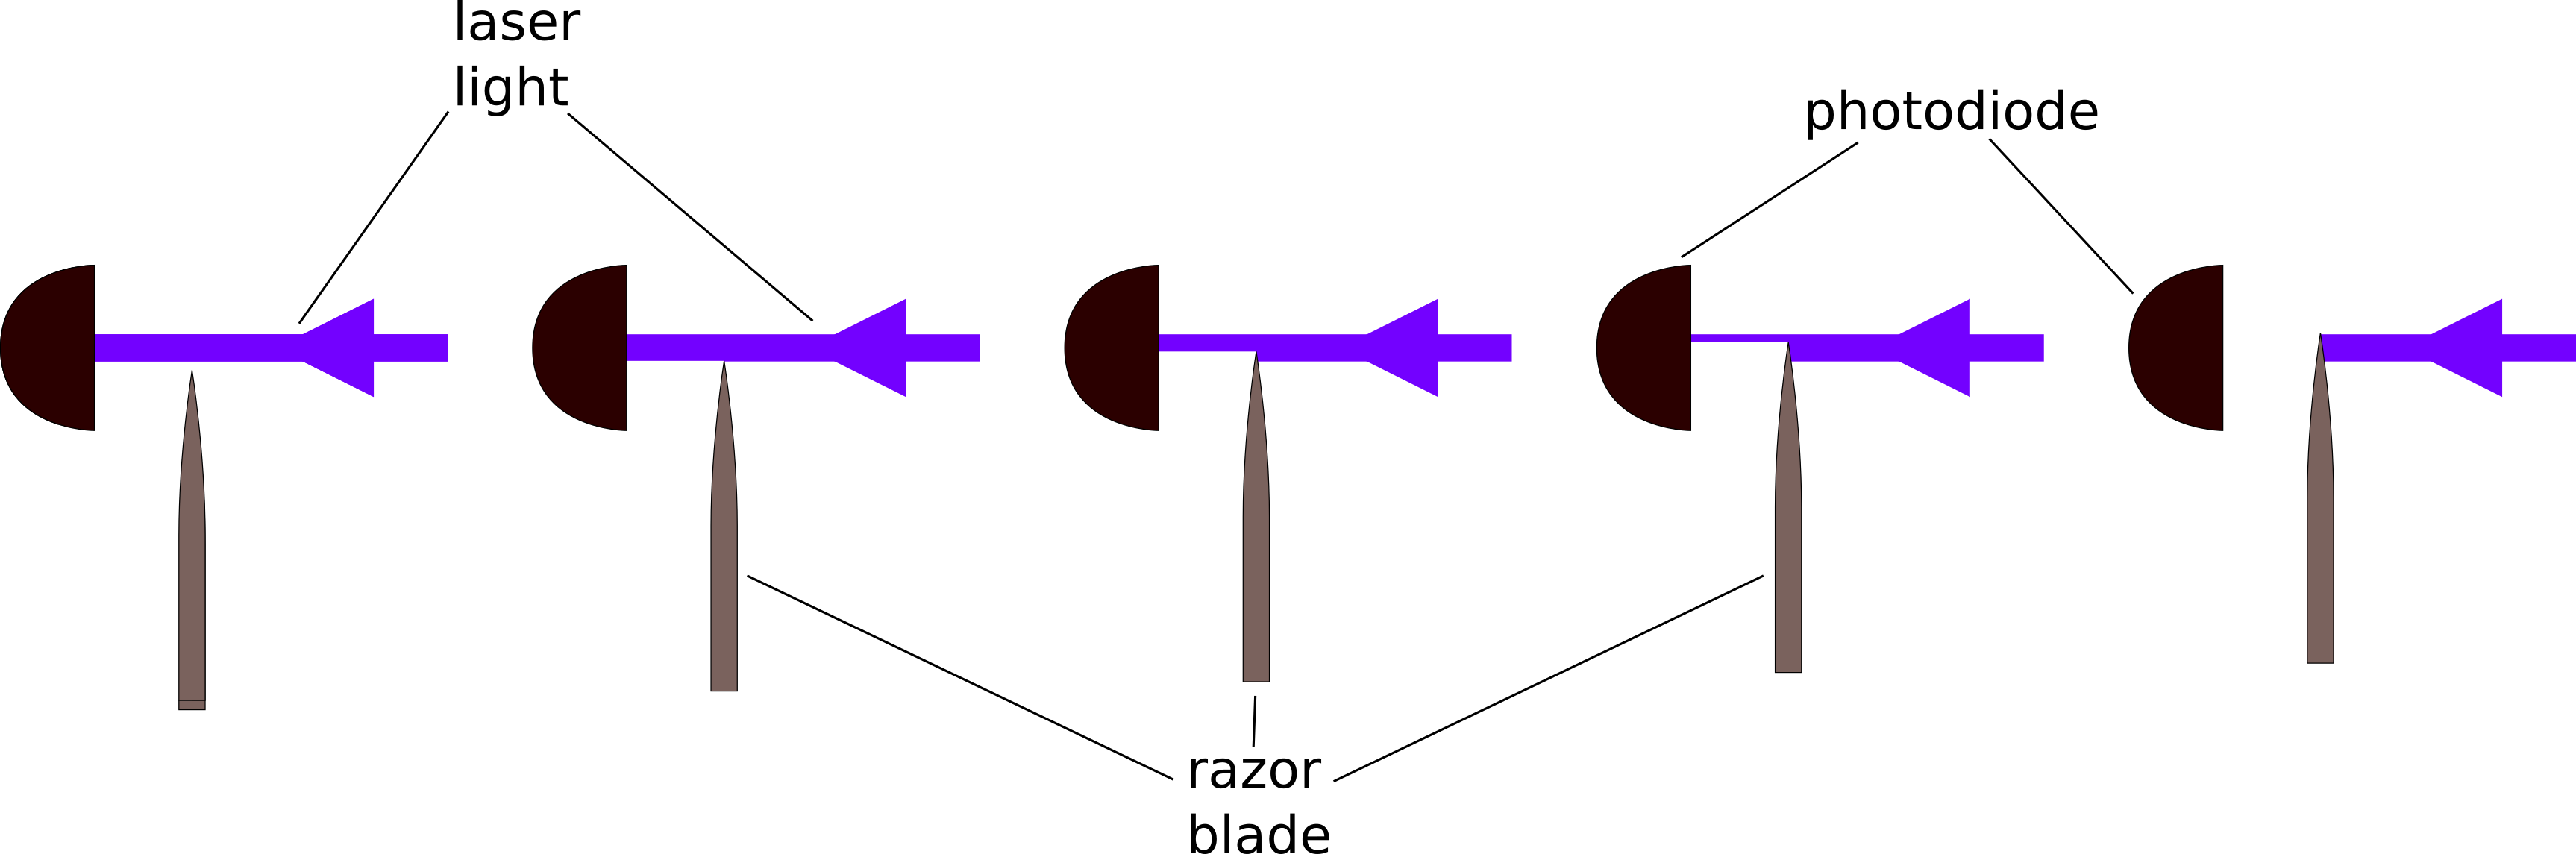
\includegraphics[width=.85\textwidth]{knife_drawing}
\caption[Knife diagram]{\label{knifeDiagram} An illustration of the razor blade method for measuring beam radius. The blade is shown in several different positions.
}
\end{figure}
If, for example, the knife is mounted vertically, the the knife would be moved in the horizontal direction. For each horizontal position, a different fraction of the beam would be occluded. 

I wrote a function called ``d4sigma'' that attempts to calculate the second moment width for arbitrary beam profiles using just the raw data taken from the photodiode and knife system. Trying to calculate D4$\sigma$ in this way is inaccurate because of how D4$\sigma$ is \emph{more} sensitive to radiation far from the center of the beam. Also, the knife technique lends itself to getting data of relatively low resolution. Finally, because I realized this and decided not to use the d4sigma function, the d4sigma function itself is not well-debugged and may be (for example) off by a constant factor.

However, if we assume a Gaussian beam profile, we can make some simplifying assumptions.
The profile for the intensity of a Gaussian beam is given by
\begin{equation} \label{electricFieldExplicitForm}
I(r,z)=I_0(z)
%\left(\frac{w_0}{w(z)}\right)^2 
\exp \left(\frac{-2 r^2}{w^2(z)}\right)
\end{equation}
where $I_0(z)$ represents the intensity at the center of the beam for any given value of $z$.
Extrapolating this to when there are two different waists in different directions, we get: 
\begin{equation}
I(r,z)= I_0\exp \left(-2\frac{x^2}{w_x^2(z)}-2\frac{y^2}{w_y^2(z)}\right) . 
\end{equation}
Now, total power ($P$) can be obtained by integrating the the intensity: 
\begin{align}
P&=\int_{-\infty}^{\infty}\int_{-\infty}^{\infty} I_0 \exp \left(-2\frac{x^2}{w_x^2(z)}-2\frac{y^2}{w_y^2(z)}\right) dx dy\\
P&=\frac{\pi}{2} I_0 w_x(z) w_y(z).
\end{align}
The equation for $I_0$ takes the form
\begin{equation}
I_0=\frac{2 P}{\pi w_x(z) w_y(z)}.
\end{equation}
%The symbol $I_0$ represents the maximum intensity that occurs within the beam (i.e. when $x=y=z=0$, or in other words, at the center of the narrowest part of the beam.)

The measurements on the photo diode correspond to the total power in the beam from $x=-\infty$ to $x_0$ where $x_0$ is the location of the knife. Thus, if we plot this power as a function of the spatial position of the knife, we expect that the result should be 
\begin{align}
P(x_0)&=\int_{\infty}^{\infty}\int_{-\infty}^{x_0} \frac{2 P}{\pi w_x(z) w_y(z)}\exp \left(-2\frac{x^2}{w_x^2(z)}-2\frac{y^2}{w_y^2(z)}\right) dx dy\\
P(x_0)&=\frac{P}{2} \left(\erf \frac{\sqrt{2} x}{W_x}+1 \right).\label{powerfitfun}
\end{align}
Eq.\,\ref{powerfitfun} can now be used as a function to which we can fit our measured data. 
%The code in masterFILEhoriz14Nov.m calculates the approximate beam waist based on a series of knife cuts. First, one loads the intensity (in arbitrary units) and the position (in the units that the waist will ultimately be given in) into a number of arrays named x1, x2, .. . etc. The user types the position of the knife along the waist (show picture) into the vector called positions. 

The program calculates the second moment width and the beam waist by assuming that the beam profile is Gaussian and finding parameters that will fit the measured data points. The function we fit to is contained in the file beamWaistCalculator, which takes as its arguments the raw position data and the raw intensity data. This function is 
\begin{equation}\label{fiterfeqn}
f(x)=a_1 \erf \left(\frac{x-a_3}{a_2}\right)+a_4.
\end{equation}
The function defined in ``beamWaistCalculator'' thus returns a vector containing $(a_1, a_2, a_3, a_4)$. In order to calculate the beam radius, we will take $a_2$ and multiply by $\sqrt{2}$. The source code to this function is included in Section\,\ref{OctaveCodeKnife}.

According to Siegman \cite{SiegmanBeamQuality}, the second moment width always propagates according to this equation: 
\begin{equation}
W_x^2(z)=W_{0x}^2 + M_x^4 \left( \frac{\lambda}{\pi W_{0x}}\right)^2 (z-z_{0x})^2. 
\end{equation}
Of course, for a Gaussian beam, we recognize that allowing $M_x^2\rightarrow 1$ gives us the equation for how the waist changes as it propagates. 
\begin{figure}
\centering
\begin{subfigure}[b]{0.47\textwidth}
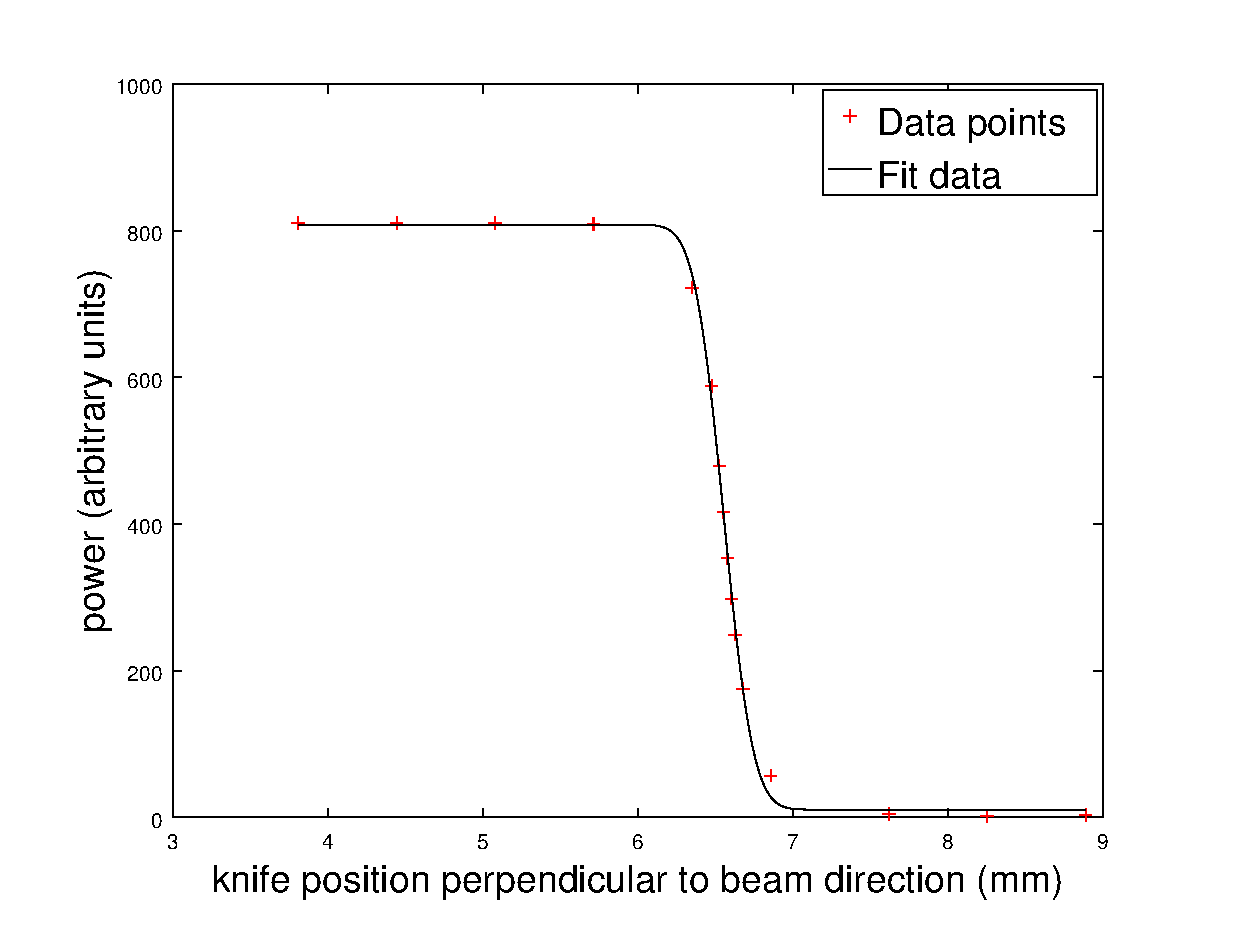
\includegraphics[width=1\textwidth]{waistFitExample.eps}
\label{waistFitExample}
\end{subfigure}
\begin{subfigure}[b]{0.47\textwidth}
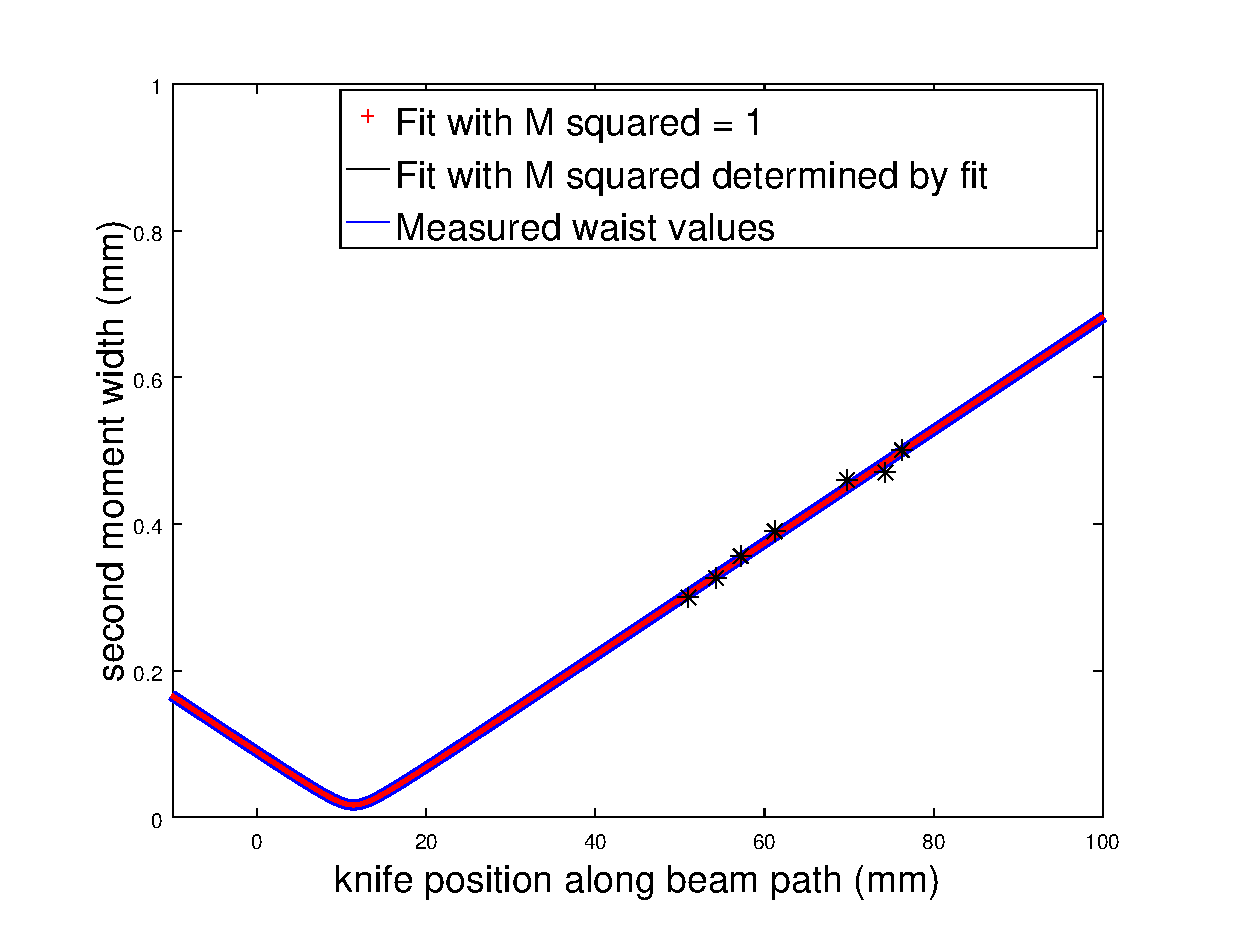
\includegraphics[width=1\textwidth]{waistExample.eps} 
\label{waistExample}
\end{subfigure}
\caption[Waist determination using a knife]{\label{waistGraphs} 
%Waist determination using a knife. On the left, there is typical data taken from a photodiode using a knife to occlude part of the beam. In general, we take data at several points along the beam path. This data is then fit to a function of the form shown in Eq.\,\ref{fiterfeqn}. This is shown on the right. The graph on the right shows a fit to equations of the form shown in Eq.\,\ref{eq:Aafinder} and \ref{eq:AAAfinder}. This data was taken for the $y$ direction on the beam going into the AOM. The fit values turn out to be $a_1=0.016875$ and $a_2=11.400$ for Eq.\,\ref{eq:Aafinder} and $a_1=1.6875e-2$, $a_2 = 11.4$, and $a_3=-2.6737e-7$ for the coefficients in Eq.\,\ref{eq:AAAfinder}. The value of $a_3$ is very small, which would suggest that $M^2\approx1$. However, because of the limited resolution and the fact that we fit the data points to a function before trying to calculate $M^2$ rather than using the directly-calculated second-moment width, we probably cannot trust the fit value corresoponding to $M^2$. On both graphs, the 0 mm point is arbitrary.
Waist determination using a knife. On the left is an example of data that was collected by measuring the beam power while occluding the beam in one direction using a razor blade. Each position on the x axis of the chart on the left corresponds to a different location of the razor blade within the beam. The curve fit to Eq.\,\ref{fiterfeqn} is also shown in the graph.
The graph on the right shows second moment widths of the beam at several points along the direction of propagation. Each data point in the graph on the right corresponds to a knife measurement taken at a different spot along the beam's direction of propagation. The fit coefficients calculated for the data in the graph on the left provides just one data point for the graph on the right. The fit to Eqs.\,\ref{eq:Aafinder} and \ref{eq:AAAfinder} is also shown in the graph on the right. 
The values of the coefficients found by fitting for the data shown turn out to be $a_1=0.016875$ and $a_2=11.400$ for the coefficients in Eq.\,\ref{eq:Aafinder} and $a_1=1.6875e-2$, $a_2 = 11.4$, and $a_3=-2.6737e-7$ for the coefficients in Eq.\,\ref{eq:AAAfinder}. The value of $a_3$ is very small, which would suggest that $M^2\approx1$. However, as mentioned in the text, I do not believe that this gives a very reliable estimate of the actual value of $M^2$. The x axis of both graphs is measured relative to an arbitrary point that was selected based on experimental convenience.
%The razor blade is mounted perpendicular to the direction of beam propagation. Each position on the x axis of the chart on the left corresponds to a different location of the razor blade within the beam. I took data like this for several positions along the direction of propagation of the beam. I then performed a fit where the fit function is of the form shown in Eq.\,\ref{fiterfeqn}. From the parameters generated by the curve fit, I extract an effective beam waist. Beam waists found in this way for several locations of the beam are shown in the plot on the right. The waist data as a function of distance along the path propagation is fitted to Eqs.\,\ref{eq:Aafinder} and \ref{eq:AAAfinder}. Allowing 
}
\end{figure}

This program then tries to fit to this:
\begin{equation}
W_x=a_1 \sqrt{1+\left(\frac{(x-a_2) \lambda}{\pi a_1^2}\right)^2}\label{eq:Aafinder},
\end{equation}
and this:
\begin{equation}
W_x=a_1 \sqrt{1+(1+a_3^2) \left(\frac{(x-a_2) \lambda}{\pi a_1^2}\right)^2}.\label{eq:AAAfinder} 
\end{equation}
Eq.\,\ref{eq:Aafinder} is very similar to Eq.\,\ref{eq:AAAfinder} except that in Eq.\,\ref{eq:Aafinder}, we are effectively forcing $M^2$ to be one. As explained in Section,\ref{optimbeamWaist}, the assumption that $M^2=1$ is a useful one since, given a set of beam radius measurements for various points along the beam, the maximum intensity calculated assuming that $M^2=1$ will always be greater than or equal to the actual intensity of the beam for any possible actual value of $M^2$. Thus, for the purposes of verifying that the intensity that we measure and calculate is below the damage threshold of the AOM, we can use the values obtained with the assumption that $M^2=1$. 

Furthermore, because the beam radii/second moment widths used to perform the curve fit described in Eqs\,\ref{eq:Aafinder} and \ref{eq:AAAfinder} were calculated assuming the beam profile is Gaussian, we do not expect to get a very good estimate of $M^2$. This is all illustrated for the $y$ dimension of a laser beam coupling into the AOM in Fig.\,\ref{waistGraphs}. Code for performing these curve fits can be found in Section\,\ref{OctaveCodeKnife}.

%power arbitrary units might be milliamps.
%it is better to get it on both sides
\section{Octave code for analyzing knife data}\label{OctaveCodeKnife}
The next two subsections contain Octave code for fitting the knife data.
\subsection{Main file}
This code completes the curve fits in Eqs.\,\ref{eq:Aafinder} and \ref{eq:AAAfinder}. It also produces one of the plots in Figure\,\ref{waistGraphs}.
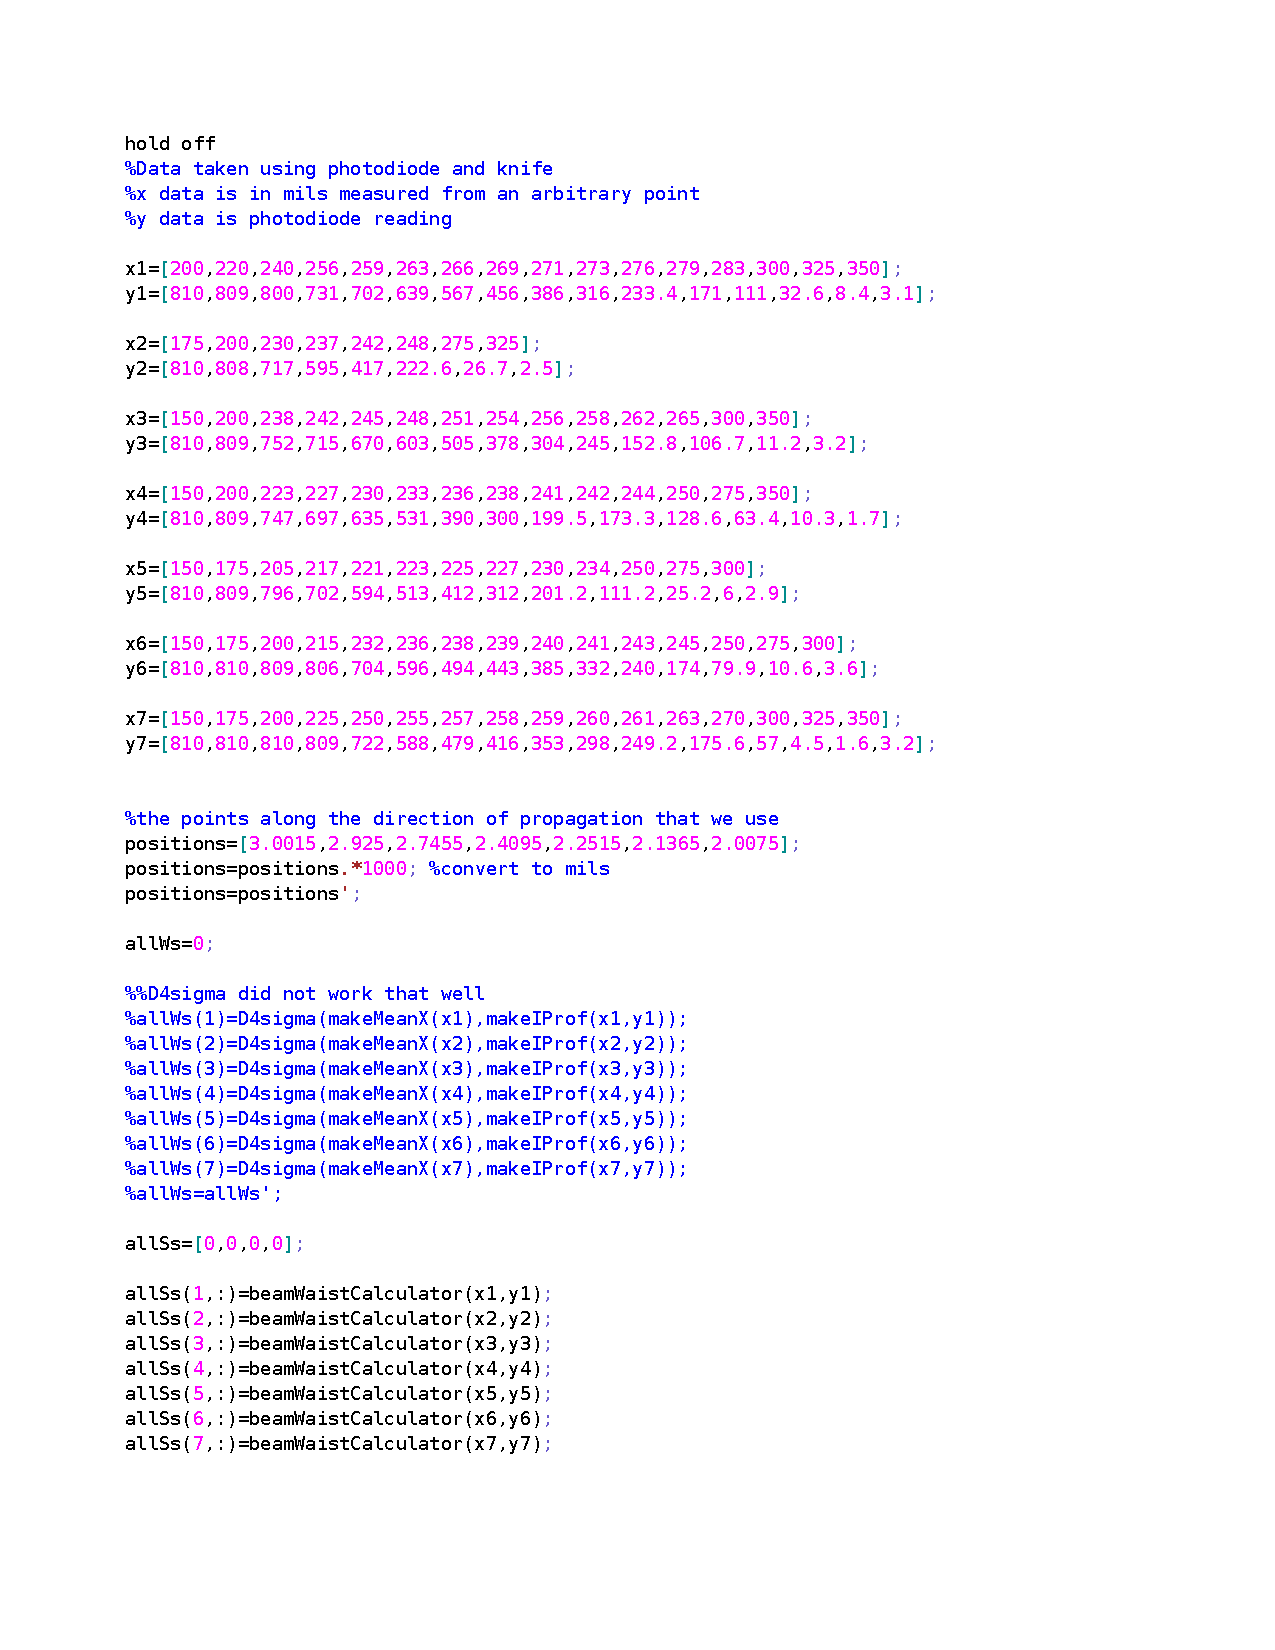
\includepdf[pages={1-2},scale=0.93]{masterFILE}
\subsection{Function beamWaistCalculator}
This is Octave code for completing the curve fit described in Eq.\,\ref{fiterfeqn}. It also produces one of the plots in Figure\,\ref{waistGraphs}. 
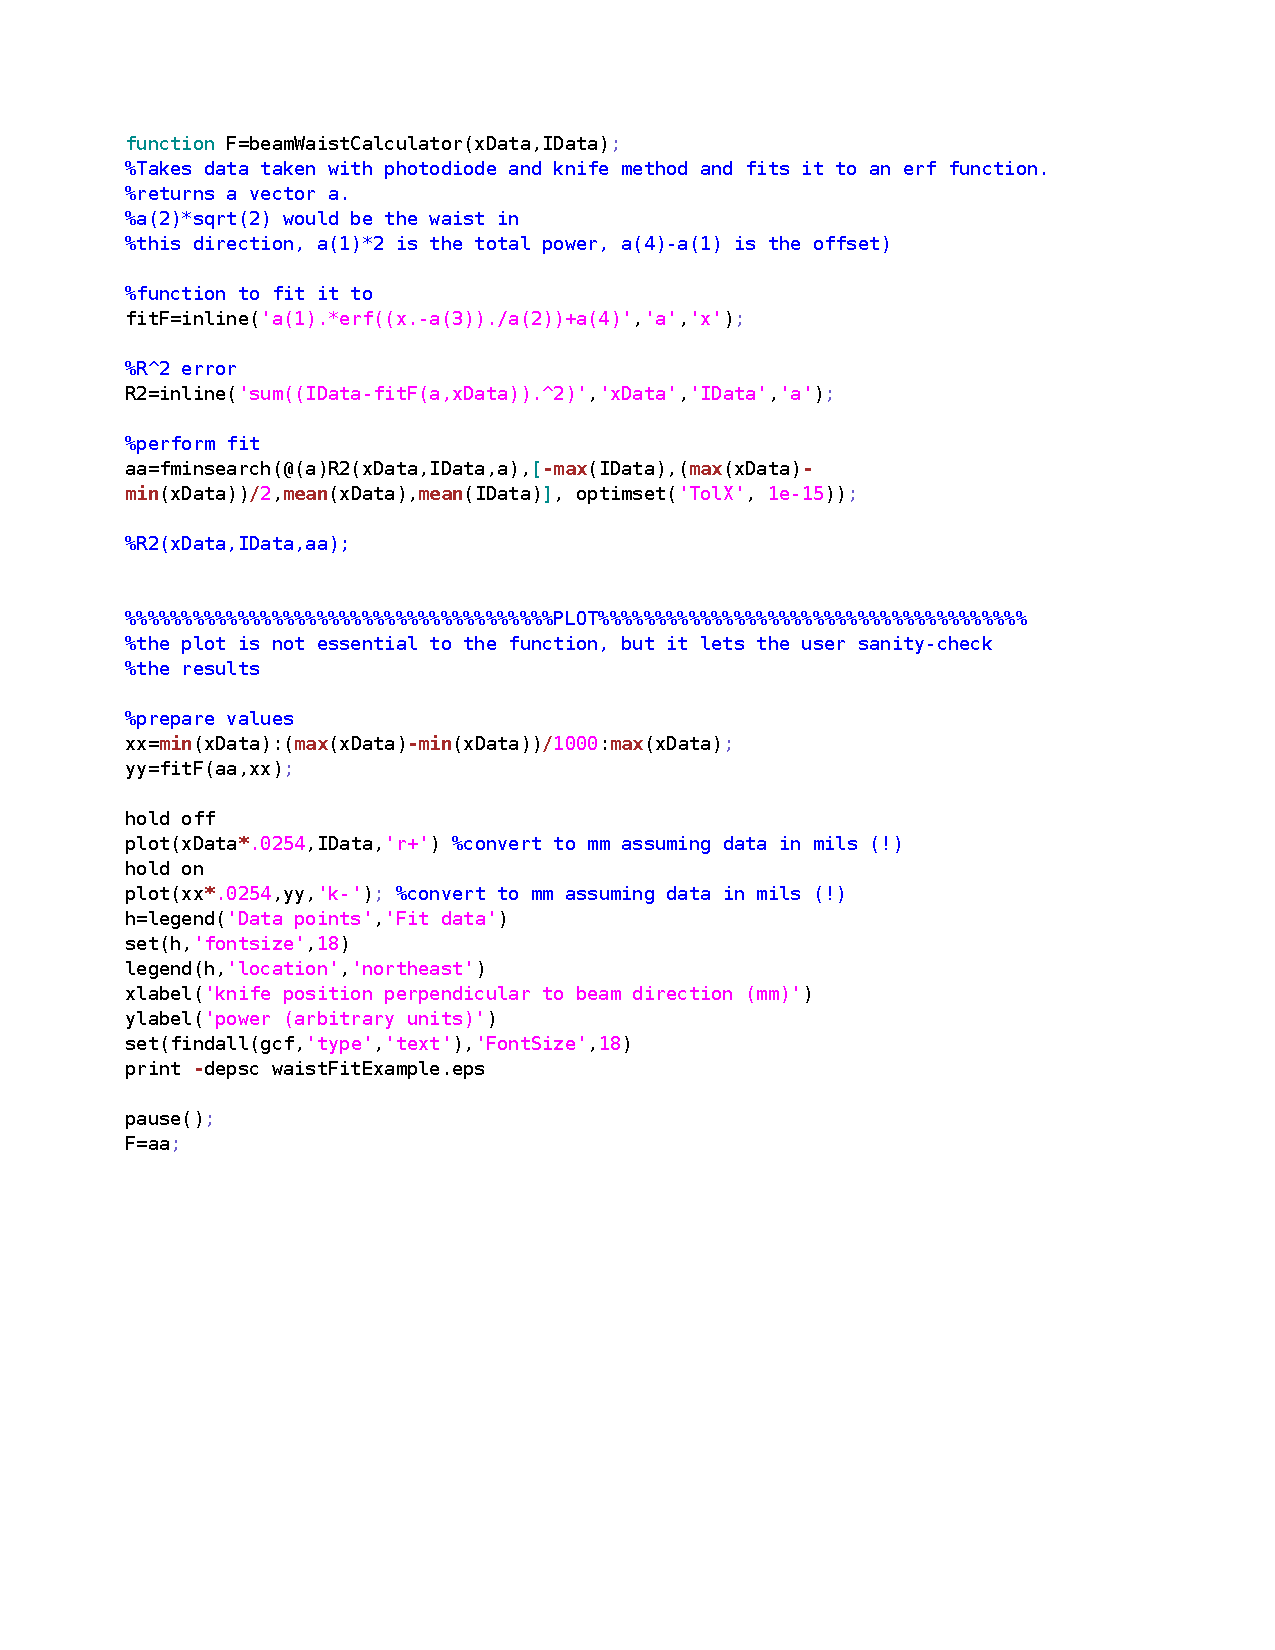
\includepdf[pages={1},scale=0.93]{beamWaist}

\section{Using the camera}
We initially wanted to measure the $M^2$ of our beam. 
The camera seems like an appealing device to use to measure beam parameters since it can take large amounts of 2D data quickly.
The measurements are hard to do accurately. The results obtained with the camera were not entirely usable.

\subsection{Investigation of feasibility of using the camera}
%insert plot of pixel count vs whatever? eh, maybe.

To investigate the camera's feasibility, we wanted to verify that the camera was (a) linear and (b) that each pixel reading was independent of the rest of the image. To this end, we took several images of the same beam, which we attenuated using the polarizing beam cube/wave plates adjustable attenuator setup described in Appendix\,\ref{twoWaveplateTrick}. We took 20 measurements. Each time we measured the total intensity of the beam using a photo diode and we took a corresponding image of the beam. Several example images are shown in Figure\,\ref{cameraimageexample}.

\begin{figure}
\centerline{
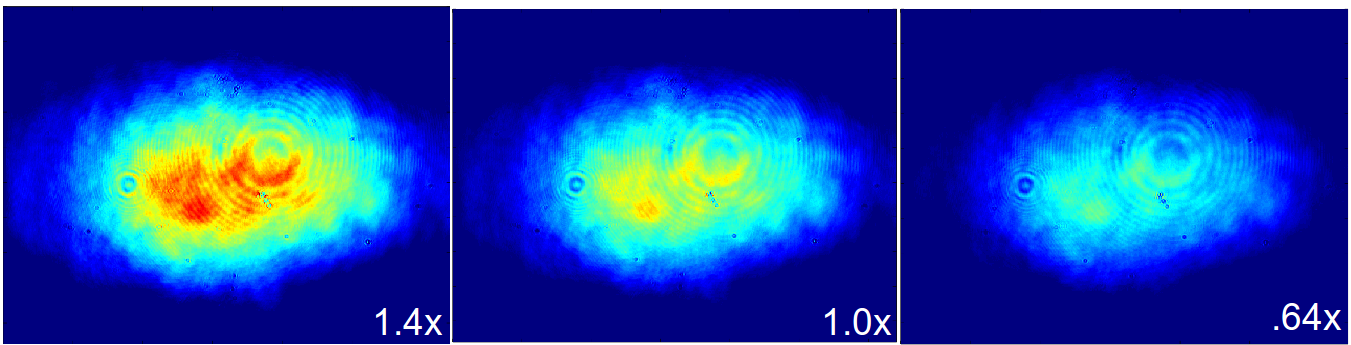
\includegraphics[width=0.95\textwidth]{cameraimage}
}
\caption[Sample camera images]{Three images taken using the camera. Each was the same laser beam with the attenuation adjusted using our wave plate and polarizer setup. The total power was measured using a photo diode and the relative total power is shown in the lower right corner of each image. By comparing the pixel values of similar spots within the image, we were able to bootstrap some calibration parameters for the camera. \label{cameraimageexample}}
\end{figure}

Our idea was that, if the camera is linear and the pixels act independently, the following statements should be true: 
\begin{itemize}
\item The ratio of the reading on any pixel to the reading on the same pixel in a different image should be equal to the ratio of the total power of the two beams used in the two readings as measured by the photo diode. 
\item Any two pixels reporting the same number of counts are experiencing the same radiance.
\end{itemize}

Thus, for example, if we see that the pixel located at $(214,442)$ has a pixel count of 127 in image 15, on which we measured the intensity to be proportional to 85.350, then we assume that we can compare it directly to a pixel located at the same location $(214,442)$ on image 20 (which had an intensity proportional to 119.70). If the reading from the $(214,442)$ pixel on image 20 was 155.46, we assume that a pixel count of 155.46 corresponds to $119.70/85.350=1.4025$ times as much intensity as a pixel count of 127. Additionally, we assume that any pixel we find in any of the images that reports a reading of 155.45 will have the same intensity as any other. 

%The Octave code created a large list of pixels along with their intensities relative to some reference pixel. The way this worked was this:
%\begin{itemize}
%\item A reference pixel is selected from one of the 20 images and added to our list of pixels.
%\item Pixels from the other 20 images whose position within their respective images matches the reference pixel's position are added to the list. Their relative intensity values are selected to be proportional to that of the reference pixel.
%\item We select a pixel from our list. Let this pixel be called $c'$
%\item We search for pixels that have nearly the same reading as $c'$, regardless of where their location is. These pixels are added to the list. Their relative intensity is set to equal the relative intensity of $c'$. This set of new pixels in the list is called $C$.
%\item For each of the pixels in $C$, we find the pixels whose position within each of the 20 images matches the position of the pixels in $C$. These, too, are added to the list. Their relative intensities are estimated by multiplying the estimated intensity of the pixel from $C$ by the relative intensity of the new pixels' image to the image containing the element of $C$.
%\item We continue to add pixels to the list.
%\end{itemize}
%From this, we bin the pixels in a grid based on what the radiance 

We went through the 20 images like this: We selected some reference pixel. We then added that pixel to a master list. We then found the corresponding pixels in the other images whose position on the grid match that of the reference pixel. They were then added to the master list, making note of their position, the reading on the pixel (count) and the assumed ratio between the amount of light hitting that pixel and the amount of light hitting reference pixel as inferred based on the readings from the photo diode.

Then, we select a random pixel from the master list and look for other pixels that have the same number of counts within any of the images. If a pixel has the same reading (number of counts) as the randomly selected pixel in the master list, it is added to the master list. Since this new pixel has the same counts as the randomly selected pixel, we assume that the pixels have the same radiance relative to the reference pixel. Once the new pixel is added to the master list, we find the corresponding pixels from the other images and add them to our list. We assume that the true radiance at these pixels is proportional to the radiance of pixel we just added. 

In this way, we create a very long list of pixels, their counts and what we have inferred about the incident illumination of each pixel by comparing it to (a) other pixels that read the same value and (b) pixels in other images of different intensities. Note that the pixels in the list are not unique. Pixels can appear multiple times in the list.

If we plot the expected pixel count (as calculated by taking the reading on the main reference pixel and multiplying it by the relative radiance factors that we've been tracking) vs the actual pixel count, we get the plot in Fig.\,\ref{cameraPixelFit}, which seems to validate the assumption of pixel independence.

However, as one can see, the camera actually has a minimum threshold below which it does not report light very well. Because the camera throws away information and has a minimum intensity threshold to register, we throw out any $M_{i j}=0$. This way our function doesn't get penalized for showing a non-zero intensity for pixels that read out zero. The number of $M_{i j}=0$ obviously doesn't change as we try different iterations of $f(M_{ij})$, so there's no way to game our little metric to make it not work.
%We did a standard fit to a 4th order polynomial and got a reasonable function to correct for the pixel values. We were a little worried about bias in the selection of pixels and things like that. We wasted some time trying to figure out how to do this better. 

We performed a curve fit to model our pixels response. In order to do this, we had to devise a cost function that produces some figure of merit to tell us whether our test function is succeeding at making all of the pixels have the right ratio. The way it works is this: Suppose that $M_{i j}$ is a big list of our pixels. The variable $j$ runs from 1 to 20, corresponding to the 20 different images, while $i$ represents all the pixels in our image.\footnote{Thus, if we are analyzing 8x8 bins, we should have 480/8*640/8=4800 pixels and i will range between 1 to 4800} Let $f(p)$ be the proposed function that takes as its argument the count on a given pixel and gives as its output something that scales with the actual intensity of the light. The figure of merit that we can use to optimize $f(p)$ is calculated as follows: 

\begin{equation}\label{fom}
{\rm Figure\:of\:merit}=\sum_{ M_{i j}\neq 0}\left(\frac{f(M_{i j})/P_j}{{\rm average\,of\,all\,nonzero\,} f(M_{i j})/P_j {\rm \,for\,the\,ith\,pixels}}-1\right)^2
\end{equation}

where $P_j$ is the power of the j th image.

In words, Eq.\,\ref{fom} can be described as follows: First, act on the pixels with the proposed function. Then, scale them according to the intensity ratios (i.e. the i th pixel in image 1 gets divided by $P_1$ while the i th pixel in image 3 gets divided by $P_3$). Then, see by what fraction the intensity of that pixel differs from the average of the intensities calculated using data from the pixels corresponding to that one. If the function really were to find the ratio perfectly, then $f(M_{ij})/P_j$ should be exactly the same for the i th pixel from each of the j images. 

We used this function to calculate what correction function to use. We did a couple of them and found great agreement with the inversion of the previous function--thus suggesting that our previous method was acceptable. 

\begin{figure}
\centerline{
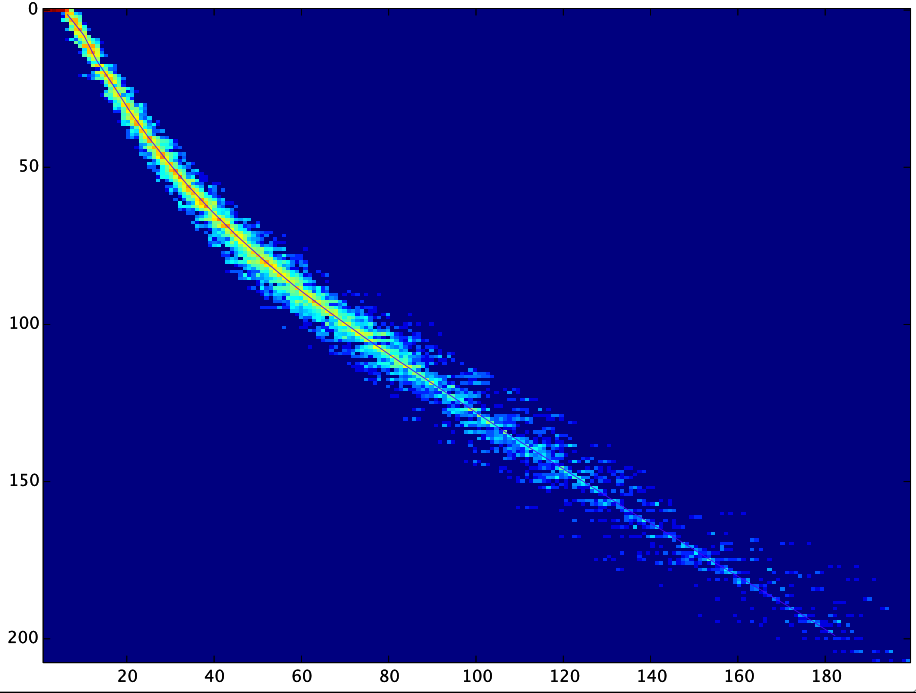
\includegraphics[width=0.95\textwidth]{cameraPixelFit}
}
\caption[Camera linearity and offset]{On the x axis is the inferred pixel reading based on our assumptions about the ratios of pixel readings. On the y axis, we can see the actual readings of the pixels. This illustrates clearly the threshold issue of the camera. In the top, left side of the plot, there is clearly a region where our inferred readings should be nonzero, but the actual readings on the camera remain at zero.\label{cameraPixelFit}}
\end{figure}

In the end, the camera offset and nonlinearity made it unsuitable for sensitive measurements of the second moment width of the beam. However they did provide a reasonable sanity check on our methods.
%\end{document}


